\documentclass[14pt,preview,border=2pt,convert={density=300,outext=.png}]{standalone}
\usepackage{amsmath}
\usepackage{graphicx}
\usepackage{hyperref}
\usepackage[latin1]{inputenc}
\usepackage{amssymb}
\usepackage{amsthm}
\usepackage{listings}
\usepackage{tikz}
\usetikzlibrary {positioning}

\begin{document}
	\begin{center}
		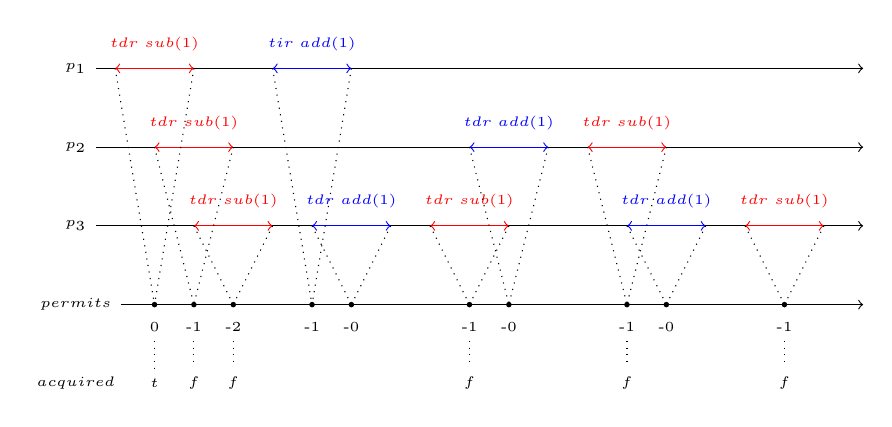
\begin{tikzpicture}
			\node (1) at (0, 4) {\tiny$p_1$};
			\node (2) [below of=1] {\tiny$p_2$};
			\node (3) [below of=2] {\tiny$p_3$};
			\node (4) [below of=3] {\tiny$permits$};
			\node (5) [below of=4] {\tiny$acquired$};
			
			\draw[->] (1) -- (10, 4);
			\draw[->] (2) -- (10, 3);
			\draw[->] (3) -- (10, 2);
			\draw[->] (4) -- (10, 1);
			
			\draw [<->, red] (.5, 4) -- node[above=1mm] {\tiny$tdr$ $sub(1)$}(1.5, 4);
			\draw [<->, blue] (2.5, 4) -- node[above=1mm] {\tiny$tir$ $add(1)$}(3.5, 4);
			
			\draw [<->, red] (1, 3) -- node[above=1mm] {\tiny$tdr$ $sub(1)$}(2, 3);
			\draw [<->, blue] (5, 3) -- node[above=1mm] {\tiny$tdr$ $add(1)$}(6, 3);
			\draw [<->, red] (6.5, 3) -- node[above=1mm] {\tiny$tdr$ $sub(1)$}(7.5, 3);
			
			\draw [<->, red] (1.5, 2) -- node[above=1mm] {\tiny$tdr$ $sub(1)$}(2.5, 2);
			\draw [<->, blue] (3, 2) -- node[above=1mm] {\tiny$tdr$ $add(1)$}(4, 2);
			\draw [<->, red] (4.5, 2) -- node[above=1mm] {\tiny$tdr$ $sub(1)$}(5.5, 2);
			\draw [<->, blue] (7, 2) -- node[above=1mm] {\tiny$tdr$ $add(1)$}(8, 2);
			\draw [<->, red] (8.5, 2) -- node[above=1mm] {\tiny$tdr$ $sub(1)$}(9.5, 2);
			
			\fill (1, 1) circle (1pt) node (6) [below=1mm] {\tiny0};
			\fill (1.5, 1) circle (1pt) node (7) [below=1mm] {\tiny-1};
			\fill (2, 1) circle (1pt) node (8) [below=1mm] {\tiny -2};
			\fill (3, 1) circle (1pt) node (9) [below=1mm] {\tiny -1};
			\fill (3.5, 1) circle (1pt) node (10) [below=1mm] {\tiny -0};
			\fill (5, 1) circle (1pt) node (11) [below=1mm] {\tiny -1};
			\fill (5.5, 1) circle (1pt) node (12) [below=1mm] {\tiny -0};
			\fill (7, 1) circle (1pt) node (13) [below=1mm] {\tiny -1};
			\fill (7.5, 1) circle (1pt) node (14) [below=1mm] {\tiny -0};
			\fill (9, 1) circle (1pt) node (15) [below=1mm] {\tiny -1};
			
			\draw[dotted] (.5, 4) -- (1, 1); \draw[dotted] (1.5, 4) -- (1, 1);
			\draw[dotted] (1, 3) -- (1.5, 1); \draw[dotted] (2, 3) -- (1.5, 1);
			\draw[dotted] (1.5, 2) -- (2, 1); \draw[dotted] (2.5, 2) -- (2, 1);
			\draw[dotted] (2.5, 4) -- (3, 1); \draw[dotted] (3.5, 4) -- (3, 1);
			\draw[dotted] (3, 2) -- (3.5, 1); \draw[dotted] (4, 2) -- (3.5, 1);
			\draw[dotted] (4.5, 2) -- (5, 1); \draw[dotted] (5.5, 2) -- (5, 1);
			\draw[dotted] (5, 3) -- (5.5, 1); \draw[dotted] (6, 3) -- (5.5, 1);
			\draw[dotted] (6.5, 3) -- (7, 1); \draw[dotted] (7.5, 3) -- (7, 1);
			\draw[dotted] (7, 2) -- (7.5, 1); \draw[dotted] (8, 2) -- (7.5, 1);
			\draw[dotted] (8.5, 2) -- (9, 1); \draw[dotted] (9.5, 2) -- (9, 1);
			
			\node (16) at (1, 0) {\tiny$t$};
			\node (17) at (1.5, 0) {\tiny$f$};
			\node (18) at (2, 0) {\tiny$f$};
			\node (19) at (5, 0) {\tiny$f$};
			\node (20) at (7, 0) {\tiny$f$};
			\node (21) at (9, 0) {\tiny$f$};

			\draw[dotted] (6) -- (16);
			\draw[dotted] (7) -- (17);
			\draw[dotted] (8) -- (18);
			\draw[dotted] (11) -- (19);
			\draw[dotted] (13) -- (20);
			\draw[dotted] (15) -- (21);
		\end{tikzpicture}
	\end{center}
\end{document}